\documentclass[11pt,letterpaper]{article}
\usepackage[utf8]{inputenc}
\usepackage[margin=2.3cm]{geometry}
\usepackage{amsmath,amssymb}
\usepackage{graphicx}
\usepackage{booktabs}
\usepackage{array}
\usepackage{rotating}
\usepackage{siunitx}
\usepackage[font=small,labelfont=bf]{caption}
\usepackage{subcaption}
\usepackage{xcolor}
\usepackage[most]{tcolorbox}
\usepackage{enumitem}
\usepackage{microtype}
\usepackage{circuitikz}
\usepackage[hidelinks]{hyperref}

\renewcommand{\figurename}{Figura}
\renewcommand{\tablename}{Tabla}
\renewcommand{\refname}{Referencias}
\renewcommand{\abstractname}{Resumen}
\renewcommand{\contentsname}{Contenido}
\sisetup{output-decimal-marker={.}, range-phrase={ a }, list-final-separator={ y }, list-pair-separator={ y }}
\definecolor{verdeclaro}{RGB}{198,239,206}
\newtcolorbox{resultado}{colback=verdeclaro,colframe=verdeclaro!60!black,boxrule=0.5pt,arc=2pt,left=6pt,right=6pt,top=4pt,bottom=4pt}
\setlist{itemsep=2pt,topsep=4pt}

\title{\textbf{Análisis y Simulación de Curva a 90° en Microcinta}\\[6pt]
\small Maestría en Ciencias en Electrónica, Universidad de Sonora.}
\date{19 de octubre de 2026}

\begin{document}
\maketitle

\begin{abstract}
Se analizó mediante simulación electromagnética de onda completa (Ansys HFSS) el efecto de cuatro discontinuidades geométricas y una de material sobre líneas de microcinta en sustrato Rogers RO4003C, entre \SI{0.1}{} y \SI{20}{GHz}. La \textbf{curva de \ang{90}} sin compensar refleja más del 1\,\% de la potencia ($|S_{11}|>-20$~dB) a partir de \SI{7.00}{GHz} y alcanza un VSWR de 2.01 a \SI{20}{GHz}. Un circuito equivalente extraído de HFSS muestra que la esquina conserva la capacitancia de un tramo recto de igual área, pero su inductancia serie es menos de la mitad, de modo que se comporta como un tramo corto de $Z_{eq}\approx\SI{32}{\ohm}$. El chaflán óptimo elimina la reflexión, pero no la radiación (\SI{5.2}{\percent} sin chaflán y \SI{4.1}{\percent} con chaflán a \SI{20}{GHz}), que se debe al cambio de dirección de la corriente. El \textbf{cambio abrupto de ancho} entre una línea de \SI{50}{\ohm} y una de \SI{100}{\ohm} se comporta de forma opuesta: su reflexión, $|\Gamma|\approx0.330$ (VSWR $\approx1.99$), está presente desde las frecuencias más bajas porque la fija el cociente de impedancias características, y cambia poco hasta \SI{20}{GHz}. Los elementos parásitos del escalón ($C\approx\SI{8.0}{fF}$ y $L\approx\SI{18}{pH}$) solo giran la fase de la reflexión unos \ang{6} a \SI{20}{GHz}. Una transición gradual de \SI{10}{mm} lleva la reflexión por debajo de $-20$~dB a partir de \SI{7.00}{GHz}, cuando su longitud supera $0.38\,\lambda_g$, pero no puede evitarla a frecuencias bajas. Ninguna de las dos variantes del cambio de ancho radia más de \SI{0.4}{\percent}, porque la corriente no cambia de dirección. El \textbf{gap en serie} interrumpe el camino de conducción: refleja casi toda la potencia desde DC, y la única transmisión es la corriente de desplazamiento a través de la capacitancia entre los extremos, que crece unos 20~dB por década. Con una separación de \SI{0.1}{mm} ($C_g\approx\SI{33}{fF}$) la transmisión pasa de \SI{-33.3}{dB} a \SI{1}{GHz} a \SI{-7.8}{dB} a \SI{20}{GHz}; al abrir el gap, $C_g$ cae a menos de \SI{1}{fF} y la capacitancia de cada extremo a tierra tiende a la de un extremo abierto. Los extremos abiertos radian del orden de 3 a 5\,\% de la potencia a \SI{20}{GHz}. En el \textbf{cambio de material} la tira continúa igual, pero sobre otro sustrato o con otro metal. Cambiar el sustrato deja intacta la inductancia por unidad de longitud y solo cambia la capacitancia, de modo que la unión es un escalón de impedancia casi ideal, $\Gamma_0=(n_1-n_2)/(n_1+n_2)$ con $n=\sqrt{\varepsilon_{\mathrm{eff}}}$: pasar a FR-4 refleja $|\Gamma|\approx0.050$ ($-26$~dB) y pasar a RO3010 ($\varepsilon_r=10.2$) refleja $|\Gamma|\approx0.243$ (VSWR $\approx1.64$) desde DC, sin radiación ni parásitos apreciables por debajo de \SI{10}{GHz}. Si el segundo material ocupa un tramo de longitud $\ell$, el efecto se vuelve significativo cuando $\ell$ supera $\lambda_g/32$. Cambiar el cobre por estaño no produce una reflexión medible ($|S_{11}|<0.006$); su efecto es distribuido: la atenuación de la línea sube 58\,\% a \SI{5}{GHz}. La \textbf{unión en T} de tres líneas de \SI{50}{\ohm} refleja un tercio de la onda desde DC, porque cada brazo ve los otros dos en paralelo; a alta frecuencia la capacitancia del cuadro de unión ($\approx\SI{75}{fF}$) y la inductancia del giro hacia la rama desequilibran el reparto, que a \SI{20}{GHz} envía el 54\,\% de la potencia de frente y el 38\,\% a la rama. Un divisor con salidas de \SI{100}{\ohm} elimina la reflexión de entrada hasta \SI{13.0}{GHz}, y una rama abierta de \SI{8}{mm} corta la transmisión a \SI{5.50}{GHz}, donde mide un cuarto de onda; esa frecuencia se predice con un error de \SI{1.8}{\percent} combinando la T, la línea y el extremo abierto de la discontinuidad 3.
\end{abstract}

\section{Objetivo}
Analizar mediante simulación el efecto que producen las discontinuidades geométricas y de material sobre la propagación de señales en una línea de microcinta, relacionando los resultados con la desadaptación de impedancias, la reflexión, la pérdida de inserción y los efectos capacitivos e inductivos parásitos. En este documento se estudian cinco: cuatro geométricas (una curva de \ang{90}, un cambio abrupto de ancho, un gap en serie y una unión en T) y un cambio de material a mitad de la línea.

\section{Pregunta de investigación}
¿Cómo afectan las discontinuidades geométricas y de material la reflexión y la transmisión de señales en interconectores de microcinta conforme aumenta la frecuencia? ¿A partir de qué región de frecuencia su efecto es significativo y cuál es la explicación electromagnética? Las Secciones~\ref{sec:d1} a~\ref{sec:d5} responden esta pregunta para cada discontinuidad, y la Sección~\ref{sec:comparacion} compara las respuestas.

\section{Marco teórico}

\subsection{La línea de microcinta}
La microcinta es una tira conductora de ancho $W$ sobre un sustrato dieléctrico de espesor $h$ y permitividad relativa $\varepsilon_r$, con un plano de tierra en la cara opuesta. Como parte del campo viaja en el aire y parte en el dieléctrico, el modo fundamental no es TEM puro sino cuasi-TEM, y se describe con una permitividad efectiva $\varepsilon_{\mathrm{eff}}$ comprendida entre 1 y $\varepsilon_r$ \cite{pozar}:
\begin{equation}
\varepsilon_{\mathrm{eff}} = \frac{\varepsilon_r+1}{2} + \frac{\varepsilon_r-1}{2}\,\frac{1}{\sqrt{1+12\,\frac{h}{W}}}.
\label{eq:eeff}
\end{equation}
La impedancia característica es
\begin{equation}
Z_0 =
\begin{cases}
\dfrac{60}{\sqrt{\varepsilon_{\mathrm{eff}}}}\ln\!\left(\dfrac{8h}{W}+\dfrac{W}{4h}\right), & W/h\leq 1,\\[12pt]
\dfrac{120\pi}{\sqrt{\varepsilon_{\mathrm{eff}}}\left[\frac{W}{h}+1.393+0.667\ln\!\left(\frac{W}{h}+1.444\right)\right]}, & W/h\geq 1,
\end{cases}
\label{eq:z0}
\end{equation}
y la longitud de onda guiada es
\begin{equation}
\lambda_g = \frac{\lambda_0}{\sqrt{\varepsilon_{\mathrm{eff}}}} = \frac{c}{f\sqrt{\varepsilon_{\mathrm{eff}}}}.
\label{eq:lg}
\end{equation}
En términos de un circuito distribuido, $Z_0=\sqrt{L'/C'}$ y la velocidad de fase es $1/\sqrt{L'C'}$, de modo que la inductancia y la capacitancia por unidad de longitud son $L'=Z_0\sqrt{\varepsilon_{\mathrm{eff}}}/c$ y $C'=\sqrt{\varepsilon_{\mathrm{eff}}}/(cZ_0)$. Una tira más angosta tiene menos capacitancia y más inductancia por unidad de longitud, y por lo tanto mayor impedancia.

\subsection{Parámetros de dispersión y figuras de mérito}
\label{sec:sparam}
Cada puerto se refiere a la impedancia de la línea conectada a él. Cuando ambas líneas son de \SI{50}{\ohm}, el coeficiente de reflexión a la entrada es simplemente $\Gamma=S_{11}$; cuando las líneas son distintas, $S_{11}$ es la reflexión que ve una onda que llega por la línea~1 si la línea~2 continúa indefinidamente, es decir, terminada en su propia impedancia. De $\Gamma$ se obtienen la razón de onda estacionaria y las pérdidas de retorno y de inserción:
\begin{equation}
\mathrm{VSWR} = \frac{1+|\Gamma|}{1-|\Gamma|}, \qquad
\mathrm{RL} = -20\log_{10}|S_{11}|, \qquad
\mathrm{IL} = -20\log_{10}|S_{21}|.
\label{eq:merito}
\end{equation}
La conservación de la energía en la red de dos puertos permite separar la potencia incidente en lo que se refleja, lo que se transmite y lo que se pierde dentro de la estructura (radiación más disipación en conductores y dieléctrico):
\begin{equation}
|S_{11}|^2 + |S_{21}|^2 + P_{\mathrm{rad}} + P_{\mathrm{dis}} = 1
\quad\Longrightarrow\quad
P \equiv 1-|S_{11}|^2-|S_{21}|^2 = P_{\mathrm{rad}} + P_{\mathrm{dis}}.
\label{eq:balance}
\end{equation}
La pérdida de inserción tiene así dos orígenes distintos: la potencia que se refleja (desadaptación) y la que se pierde ($P$). La parte debida solo a la reflexión es $\mathrm{IL}_{\mathrm{refl}}=-10\log_{10}\left(1-|S_{11}|^2\right)$.

\subsection{Discontinuidades y su circuito equivalente}
En una discontinuidad el campo no puede satisfacer las condiciones de frontera solo con el modo cuasi-TEM; se excitan además modos de orden superior que están por debajo de su frecuencia de corte y decaen rápidamente con la distancia. Estos modos evanescentes no transportan potencia, pero almacenan energía eléctrica $W_e$ y magnética $W_m$ en la vecindad de la discontinuidad. Por el teorema de Poynting complejo, la impedancia que ve la línea es \cite{pozar}
\begin{equation}
Z = \frac{P_\ell + 2j\omega\left(W_m - W_e\right)}{\frac{1}{2}|I|^2},
\label{eq:poynting}
\end{equation}
de modo que un exceso de energía eléctrica se manifiesta como una capacitancia y un exceso de energía magnética como una inductancia. Mientras la discontinuidad sea pequeña frente a $\lambda_g$, estas energías se pueden representar con elementos concentrados.

\paragraph{Curva de \ang{90}.} El modelo clásico es una red en T con una inductancia $L$ en cada rama serie y una capacitancia $C$ en paralelo \cite{gupta}. A primer orden en $\omega$, la matriz $ABCD$ de esa red es $\begin{pmatrix}1 & 2j\omega L\\ j\omega C & 1\end{pmatrix}$, y el coeficiente de reflexión resulta
\begin{equation}
S_{11} \approx \frac{j\omega}{2}\left(\frac{2L}{Z_0} - C Z_0\right)
\quad\Longrightarrow\quad
|\Gamma| \approx \frac{\omega\tau}{2}, \qquad \tau \equiv C Z_0 - \frac{2L}{Z_0}.
\label{eq:gamma_tau}
\end{equation}
Un tramo uniforme de línea de \SI{50}{\ohm} tiene $C Z_0 = 2L/Z_0$ y no refleja. La curva refleja porque rompe ese equilibrio, y \eqref{eq:gamma_tau} anticipa dos cosas: $|\Gamma|$ crece proporcionalmente a la frecuencia, y el signo de $\tau$ indica si la discontinuidad es capacitiva ($\tau>0$, $S_{11}$ en la mitad inferior de la carta de Smith) o inductiva. Una forma equivalente de verlo es asignar a la esquina una impedancia local $Z_{eq}=\sqrt{2L/C}$: si $Z_{eq}<Z_0$, la esquina actúa como un tramo corto de menor impedancia.

\subsection{Compensación}
\paragraph{Chaflán.} La compensación habitual de la curva es recortar la esquina exterior. Douville y James determinaron experimentalmente el porcentaje óptimo de recorte de la diagonal \cite{douville}:
\begin{equation}
M = 52 + 65\,e^{-1.35\,W/h}\ \ (\%).
\label{eq:miter}
\end{equation}

\paragraph{Transición gradual.} Un cambio de ancho no se puede compensar con un recorte, porque su reflexión principal no viene de los parásitos sino de la diferencia de impedancias. Lo que sí se puede hacer es repartir el cambio a lo largo de una longitud $L_t$. En una transición exponencial, $\ln Z$ varía linealmente con la posición, $Z(x)=Z_1\exp\!\left[\frac{x}{L_t}\ln\frac{Z_2}{Z_1}\right]$, y el coeficiente de reflexión es \cite{pozar}
\begin{equation}
\Gamma = \frac{1}{2}\ln\!\left(\frac{Z_2}{Z_1}\right) e^{-j\beta L_t}\,\frac{\sin\beta L_t}{\beta L_t}.
\label{eq:taper}
\end{equation}
A baja frecuencia ($\beta L_t\to 0$) refleja lo mismo que el escalón; $|\Gamma|$ se anula por primera vez cuando $\beta L_t=\pi$, es decir, cuando $L_t=\lambda_g/2$.

\section{Metodología común}

\subsection{Sustrato y diseño de las líneas}
\label{sec:diseno}
Se eligió el laminado Rogers RO4003C, con $h=\SI{0.508}{mm}$, $\varepsilon_r=3.55$ y $\tan\delta=0.0027$, y conductores de cobre \cite{rogers}. Para la línea de \SI{50}{\ohm} ($W/h>2$), la síntesis de \cite{pozar} da
\begin{gather}
B = \frac{377\pi}{2Z_0\sqrt{\varepsilon_r}} = 6.286, \nonumber\\[4pt]
\frac{W}{h} = \frac{2}{\pi}\left[B-1-\ln(2B-1)+\frac{\varepsilon_r-1}{2\varepsilon_r}\left(\ln(B-1)+0.39-\frac{0.61}{\varepsilon_r}\right)\right] = 2.237,
\label{eq:sintesis}
\end{gather}
es decir, $W=\SI{1.136}{mm}$, que se redondeó a $W=W_1=\SI{1.14}{mm}$. Con este valor, \eqref{eq:eeff} y \eqref{eq:z0} dan
\[
\varepsilon_{\mathrm{eff}} = 2.781, \qquad Z_0 = \SI{50.15}{\ohm},
\]
y por \eqref{eq:lg} la longitud de onda guiada es $\lambda_g=\SI{17.99}{mm}$ a \SI{10}{GHz} y $\lambda_g=\SI{8.99}{mm}$ a \SI{20}{GHz}. Para la línea de \SI{100}{\ohm} de la discontinuidad 2 ($W/h<2$) la síntesis es
\begin{equation}
A = \frac{Z_0}{60}\sqrt{\frac{\varepsilon_r+1}{2}} + \frac{\varepsilon_r-1}{\varepsilon_r+1}\left(0.23+\frac{0.11}{\varepsilon_r}\right) = 2.660, \qquad
\frac{W}{h} = \frac{8e^A}{e^{2A}-2} = 0.565,
\label{eq:sintesis100}
\end{equation}
es decir, $W=\SI{0.287}{mm}$, redondeado a $W_2=\SI{0.29}{mm}$, con $\varepsilon_{\mathrm{eff}}=2.547$ y $Z_0=\SI{99.6}{\ohm}$.

\subsection{Configuración de la simulación}
\label{sec:config}
Se usó Ansys Electronics Desktop Student 2025~R2 (HFSS, solución \emph{Driven Modal}). Todos los modelos se generaron con scripts de automatización, de modo que comparten exactamente la misma configuración:
\begin{itemize}
\item \textbf{Conductores:} láminas de espesor cero con conductividad finita de cobre para la traza y el plano de tierra (en la discontinuidad 4, uno de los casos lleva estaño en la segunda mitad de la traza).
\item \textbf{Frontera abierta:} caja de aire con frontera de radiación, a \SI{7}{mm} del borde de la traza más ancha a los lados y con altura total $14h=\SI{7.1}{mm}$.
\item \textbf{Puertos:} puertos de onda de un modo, de ancho $P_w=5W_1=\SI{5.7}{mm}$ y altura $8h=\SI{4.06}{mm}$, iguales en todos los diseños. El ancho se limitó para que el primer modo de caja del puerto, cuya frecuencia de corte se estima como $f_c\approx c/\left(2P_w\sqrt{\varepsilon_\perp}\right)\approx\SI{25}{GHz}$ con $\varepsilon_\perp=\frac{8h}{7h+h/\varepsilon_r}$, quede fuera de la banda.
\item \textbf{Normalización y de-embedding:} en la curva, ambos puertos están sobre líneas de \SI{50}{\ohm} y los parámetros $S$ se renormalizaron a \SI{50}{\ohm}. En las demás discontinuidades cada puerto se dejó referido a la impedancia de su propia línea (Sección~\ref{sec:sparam}); renormalizar el puerto de la línea de \SI{100}{\ohm} a \SI{50}{\ohm} agregaría una segunda reflexión que no existe en el circuito real. En ambos casos los planos de referencia se desplazaron hacia adentro hasta la discontinuidad.
\item \textbf{Malla y barrido:} refinamiento adaptativo a \SI{20}{GHz} hasta $\max|\Delta S|<0.005$ en dos pases consecutivos, y barrido interpolante de \SI{0.1}{} a \SI{20}{GHz} con paso de \SI{50}{MHz}.
\item \textbf{Gemelos sin pérdidas:} de cada estructura se simuló además una copia con conductores perfectos y $\tan\delta=0$, cuyo uso se explica en la Sección~\ref{sec:validacion}.
\end{itemize}
La Tabla~\ref{tab:conv} resume la convergencia. La versión estudiantil limita el tamaño de la malla, y todos los diseños quedaron por debajo de ese límite. Solo la transición gradual sin pérdidas, la estructura más larga, se detuvo en el pase 14 (\num{51971} elementos), porque el pase siguiente (\num{70962} elementos) excedía el límite; en ese pase ya cumplía el criterio de convergencia. En el gap, cinco diseños llegaron al máximo de 15 pases con un solo pase bajo el criterio; su último $\max|\Delta S|$ es a lo sumo 0.0054, y los gemelos con y sin pérdidas dan los mismos parámetros del circuito dentro de la incertidumbre. Los 16 diseños del cambio de material y los 10 de la unión en T convergieron con el criterio completo, con a lo sumo \num{46786} elementos; el divisor sin pérdidas lo hizo en el último pase permitido.

\begin{table}[htbp]
\centering
\caption{Convergencia de la malla adaptativa.}
\label{tab:conv}
\footnotesize
\renewcommand{\arraystretch}{0.86}
\begin{tabular}{lccc}
\toprule
Diseño & Pases & Elementos & $\max|\Delta S|$ final \\
\midrule
\multicolumn{4}{l}{\textit{Discontinuidad 1: curva de \ang{90}}} \\
Referencia & 11 & \num{14911} & 0.0029 \\
Curva sin chaflán & 14 & \num{23962} & 0.0045 \\
Curva con chaflán & 10 & \num{11127} & 0.0025 \\
Referencia sin pérdidas & 10 & \num{11485} & 0.0042 \\
Curva sin chaflán, sin pérdidas & 13 & \num{20687} & 0.0045 \\
Curva con chaflán, sin pérdidas & 13 & \num{24533} & 0.0030 \\
\midrule
\end{tabular}
\end{table}

\subsection{Validación del modelo y tratamiento del error numérico}
\label{sec:validacion}
Una primera versión del modelo (caja de aire con \SI{4}{mm} de margen y $8h$ de altura, criterio $\max|\Delta S|<0.02$) reproducía bien $S_{11}$ de la curva, pero el balance \eqref{eq:balance} de la línea recta mostraba una pérdida aparente de hasta 4\,\%, demasiado alta para un tramo de \SI{1.14}{mm}. Para encontrar su origen se simularon variantes de la referencia que aíslan una causa a la vez (Tabla~\ref{tab:diag}):
\begin{itemize}
\item La variante sin pérdidas conserva casi toda la pérdida aparente, así que no es pérdida física sino un artefacto del modelo.
\item Sin de-embedding la pérdida aumenta en \SI{1.8}{\percent} (\SI{0.08}{dB}) a \SI{10}{GHz}, del orden de la pérdida de cobre y dieléctrico estimada para los \SI{12}{mm} de alimentación (\SI{0.09}{dB}). El de-embedding funciona correctamente.
\item Agrandar la caja de aire reduce el artefacto: la frontera de radiación demasiado cercana absorbía parte del campo cercano de la línea.
\item Refinar la malla cambió poco el resultado: el residuo que queda proviene de la transición entre el puerto, que tiene bordes conductores, y la línea abierta que lo rodea.
\end{itemize}

\begin{table}[htbp]
\centering
\caption{Pérdida aparente $P=1-|S_{11}|^2-|S_{21}|^2$ de la línea de referencia de la curva a \SI{10}{GHz} en las variantes de diagnóstico.}
\label{tab:diag}
\small
\begin{tabular}{llc}
\toprule
Variante & Cambio respecto al modelo inicial & $P$ (\%) \\
\midrule
Inicial & caja de \SI{4}{mm} y $8h$, $\max|\Delta S|<0.02$ & 4.00 \\
R2 & sin pérdidas (PEC, $\tan\delta=0$) & 3.57 \\
R3 & sin de-embedding & 5.77 \\
R4 & caras de los puertos conductoras & 3.65 \\
R5 & caja de \SI{7}{mm} y $14h$ & 2.65 \\
R6 & R5 + caras conductoras & 1.64 \\
R7 & R6 sin pérdidas & 1.10 \\
Final & caja de \SI{7}{mm} y $14h$, $\max|\Delta S|<0.005$ & 2.77 \\
Final sin pérdidas & gemelo sin pérdidas del modelo final & 2.10 \\
\bottomrule
\end{tabular}
\end{table}

Ese residuo es común a todas las estructuras, porque todas tienen los mismos puertos y la misma alimentación. Por eso se eliminó por diferencia, usando los gemelos sin pérdidas. Si $P_X$ es la pérdida aparente de la estructura $X$ y $P_{X0}$ la de su gemelo sin pérdidas, entonces
\begin{equation}
P_{\mathrm{rad}} = P_{X0} - P_{A0}, \qquad P_{\mathrm{dis}} = P_X - P_{X0},
\label{eq:separacion}
\end{equation}
donde $A0$ es la referencia sin pérdidas. Por debajo de \SI{6}{GHz} la radiación de la curva debe ser nula, y ahí \eqref{eq:separacion} da valores dentro de $\pm\SI{0.2}{\percent}$, que se toma como la incertidumbre de $P_{\mathrm{rad}}$. Por la misma razón, el nivel de $|S_{11}|$ de la referencia (alrededor de $-30$ a \SI{-45}{dB}) es el piso por debajo del cual no se puede resolver la reflexión de una discontinuidad. En las demás discontinuidades se dio un paso más y el mismo residuo se quitó de los parámetros $S$ completos (Sección~\ref{sec:correccion}).

\subsection{Extracción del circuito equivalente de la curva}
\label{sec:extraccion}
Como las estructuras de la curva son simétricas y recíprocas ($S_{22}=S_{11}$, $S_{12}=S_{21}$), los parámetros $S$ se convirtieron a parámetros $Z$,
\begin{equation}
Z_{11} = Z_0\,\frac{(1+S_{11})(1-S_{22})+S_{12}S_{21}}{\Delta}, \qquad
Z_{21} = Z_0\,\frac{2S_{21}}{\Delta}, \qquad
\Delta = (1-S_{11})(1-S_{22})-S_{12}S_{21},
\label{eq:zparam}
\end{equation}
y de ellos se obtuvieron los elementos de la red en T de cada estructura,
\begin{equation}
C = -\frac{1}{\omega\,\mathrm{Im}\{Z_{21}\}}, \qquad
L = \frac{\mathrm{Im}\{Z_{11}-Z_{21}\}}{\omega}, \qquad
Z_{eq} = \sqrt{\frac{2L}{C}}.
\label{eq:LC}
\end{equation}
Para la referencia estos valores corresponden simplemente al tramo recto de longitud $W$ que queda entre los planos de referencia, lo que permite comparar la esquina contra un tramo recto de la misma área de metal. El cambio de ancho requiere otro procedimiento, que se describe en la Sección~\ref{sec:ajuste}.

%======================================================================
\section{Discontinuidad 1: curva de \ang{90}}
\label{sec:d1}

\subsection{Estructuras simuladas}
Se construyeron las tres estructuras de la Figura~\ref{fig:geo}, con la misma línea, el mismo sustrato y la misma caja de simulación:
\begin{itemize}
\item \textbf{Referencia:} línea recta de longitud $2L_1+W$, con $L_1=\SI{6}{mm}$. Es el caso ``Puerto 1 $\rightarrow$ línea uniforme de \SI{50}{\ohm} $\rightarrow$ Puerto 2'' que pide el proyecto.
\item \textbf{Curva de \ang{90}:} dos tramos de longitud $L_1$ unidos por una esquina cuadrada de $W\times W$, de modo que la longitud del eje es la misma que la de la referencia.
\item \textbf{Curva con chaflán:} la misma curva con la esquina exterior recortada según \eqref{eq:miter}, que da $M=55.1\,\%$; se usó $M=55\,\%$.
\end{itemize}

\begin{figure}[htbp]
\centering
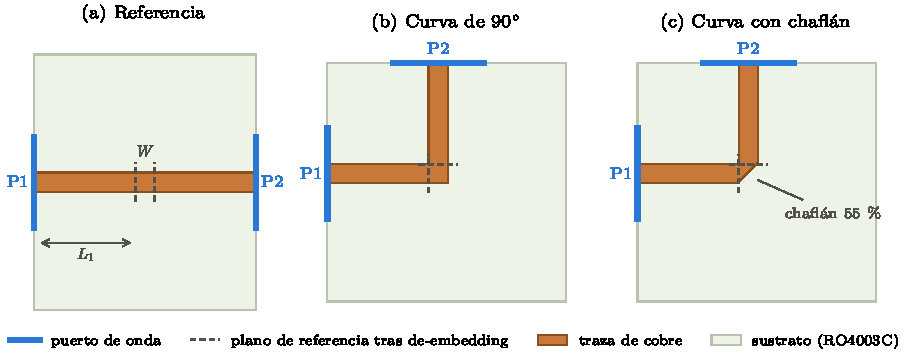
\includegraphics[width=\textwidth]{figuras/fig0_geometria.pdf}
\caption{Vista superior de las estructuras de la curva. Los planos de referencia (líneas punteadas) quedan, tras el de-embedding de $L_1$, en los bordes de la esquina; en la referencia encierran un tramo recto de longitud $W$.}
\label{fig:geo}
\end{figure}

La Figura~\ref{fig:hfss3d} muestra los modelos tal como quedaron construidos en HFSS: la traza de cobre sobre el sustrato, el plano de tierra en la cara inferior, los dos puertos de onda en las caras laterales y la caja de aire que cierra el dominio.

\begin{figure}[htbp]
\centering
\begin{subfigure}[b]{0.325\textwidth}
\centering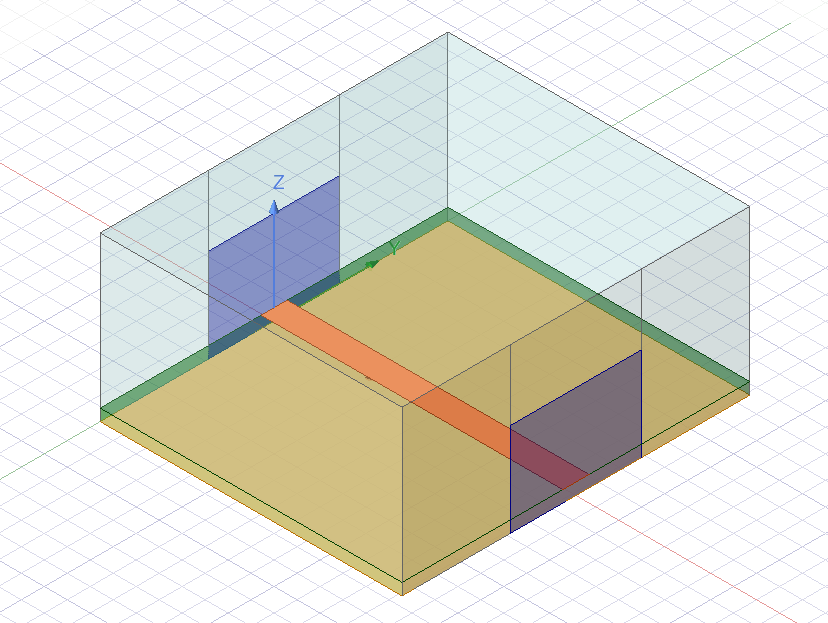
\includegraphics[width=\linewidth]{figuras/hfss3d_referencia.png}
\caption{Referencia}
\end{subfigure}\hfill
\begin{subfigure}[b]{0.325\textwidth}
\centering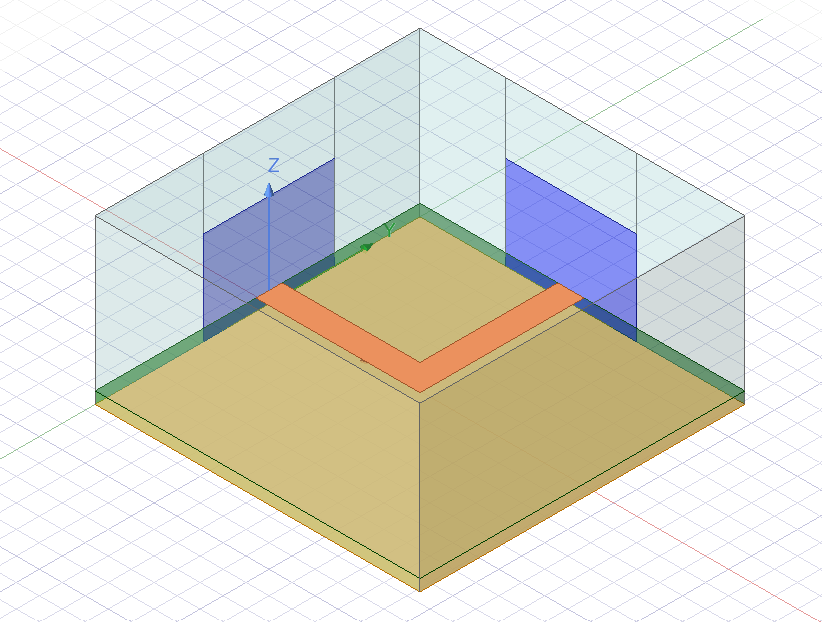
\includegraphics[width=\linewidth]{figuras/hfss3d_curva.png}
\caption{Curva de \ang{90}}
\end{subfigure}\hfill
\begin{subfigure}[b]{0.325\textwidth}
\centering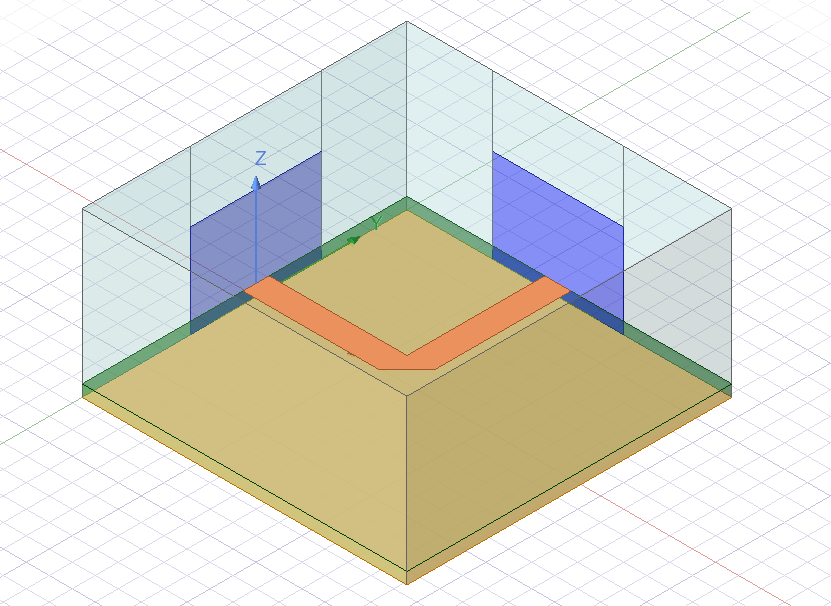
\includegraphics[width=\linewidth]{figuras/hfss3d_chaflan.png}
\caption{Curva con chaflán}
\end{subfigure}
\caption{Modelos 3D de la curva en HFSS. En naranja la traza, en azul los puertos de onda; el bloque inferior es el sustrato con el plano de tierra y el volumen transparente es la caja de aire con frontera de radiación.}
\label{fig:hfss3d}
\end{figure}

\subsection{Resultados}

\subsubsection{Reflexión}
La Figura~\ref{fig:s11} compara $|S_{11}|$ de las tres estructuras y la Tabla~\ref{tab:sparam} resume los valores en frecuencias seleccionadas. La referencia se mantiene por debajo de \SI{-30.5}{dB} en toda la banda, lo que valida el montaje. La curva sin compensar crece monotónicamente con la frecuencia, cruza \SI{-30}{dB} a \SI{3.90}{GHz}, \SI{-20}{dB} a \SI{7.00}{GHz} y llega a \SI{-9.5}{dB} a \SI{20}{GHz}. La curva con chaflán no supera \SI{-30.7}{dB} en ningún punto, es decir, queda al nivel de la propia referencia.

\begin{figure}[htbp]
\centering
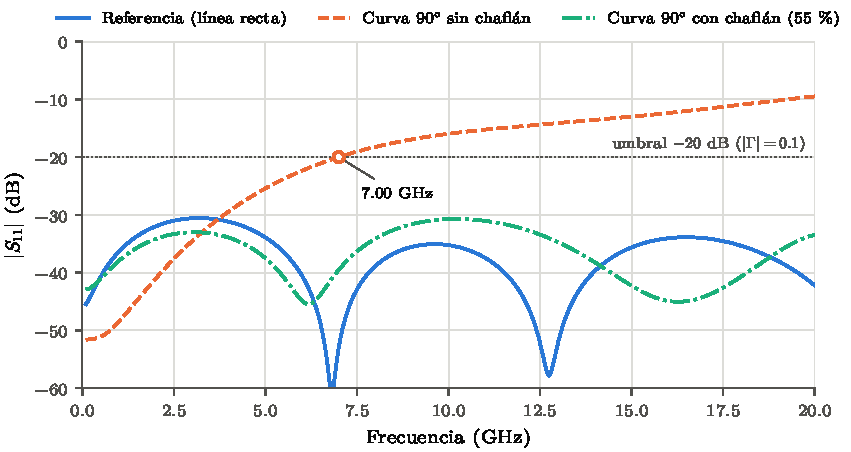
\includegraphics[width=\textwidth]{figuras/fig1_S11_dB.pdf}
\caption{Curva de \ang{90}: magnitud de $S_{11}$. El punto marca la frecuencia a la que la curva sin compensar supera el umbral de $-20$~dB ($|\Gamma|=0.1$, VSWR $=1.22$, 1\,\% de la potencia reflejada).}
\label{fig:s11}
\end{figure}

\begin{figure}[htbp]
\centering
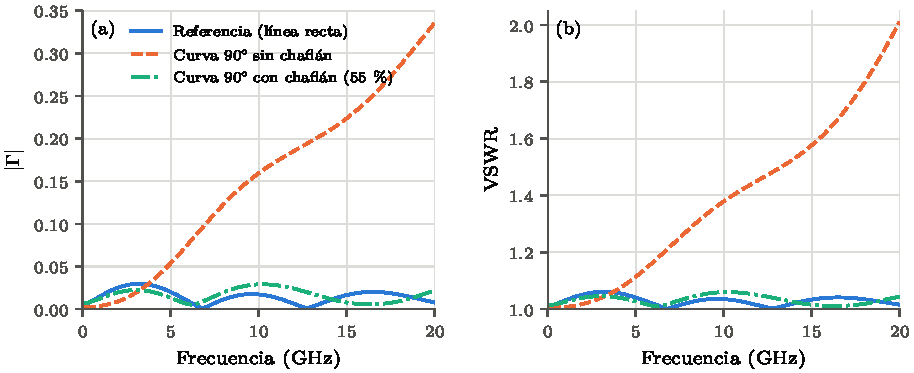
\includegraphics[width=\textwidth]{figuras/fig3_Gamma_VSWR.pdf}
\caption{Curva de \ang{90}: (a) magnitud del coeficiente de reflexión y (b) VSWR.}
\label{fig:gamma}
\end{figure}

La Figura~\ref{fig:gamma} muestra lo mismo en términos de $|\Gamma|$ y VSWR. A \SI{20}{GHz} la curva sin compensar tiene $|\Gamma|=0.336$ y VSWR $=2.01$, mientras que la curva con chaflán se mantiene en VSWR $\leq 1.06$ en toda la banda.

\begin{table}[htbp]
\centering
\caption{Curva de \ang{90}: parámetros de dispersión en frecuencias seleccionadas.}
\label{tab:sparam}
\small
\setlength{\tabcolsep}{3.2pt}
\begin{tabular}{c cccc cccc cccc}
\toprule
 & \multicolumn{4}{c}{Referencia} & \multicolumn{4}{c}{Curva sin chaflán} & \multicolumn{4}{c}{Curva con chaflán} \\
\cmidrule(lr){2-5}\cmidrule(lr){6-9}\cmidrule(lr){10-13}
$f$ (GHz) & $S_{11}$ & $|\Gamma|$ & VSWR & $S_{21}$ & $S_{11}$ & $|\Gamma|$ & VSWR & $S_{21}$ & $S_{11}$ & $|\Gamma|$ & VSWR & $S_{21}$ \\
 & (dB) & & & (dB) & (dB) & & & (dB) & (dB) & & & (dB) \\
\midrule
2 & -32.0 & 0.025 & 1.05 & -0.03 & -41.0 & 0.009 & 1.02 & -0.03 & -34.2 & 0.020 & 1.04 & -0.03 \\
5 & -33.9 & 0.020 & 1.04 & -0.09 & -25.4 & 0.054 & 1.11 & -0.09 & -37.5 & 0.013 & 1.03 & -0.08 \\
10 & -35.2 & 0.017 & 1.04 & -0.12 & -15.9 & 0.159 & 1.38 & -0.26 & -30.7 & 0.029 & 1.06 & -0.14 \\
15 & -35.6 & 0.017 & 1.03 & -0.12 & -13.0 & 0.224 & 1.58 & -0.45 & -42.3 & 0.008 & 1.02 & -0.22 \\
20 & -42.2 & 0.008 & 1.02 & -0.08 & -9.5 & 0.336 & 2.01 & -0.87 & -33.4 & 0.021 & 1.04 & -0.26 \\
\bottomrule
\end{tabular}
\end{table}

\subsubsection{Carácter de la reflexión y circuito equivalente}
En la carta de Smith (Figura~\ref{fig:smith}) la trayectoria de $S_{11}$ de la curva sin compensar arranca cerca del centro, cae a la mitad inferior con un ángulo de \ang{-95.6} a \SI{5}{GHz} y se aleja del centro al aumentar la frecuencia. Por \eqref{eq:gamma_tau}, un ángulo cercano a \ang{-90} identifica una discontinuidad predominantemente capacitiva. Las simulaciones con y sin pérdidas dan prácticamente la misma $S_{11}$ (diferencia máxima de \SI{0.1}{dB} entre 3 y \SI{20}{GHz}), lo que confirma que la reflexión es reactiva: proviene de energía almacenada y no de energía disipada.

\begin{figure}[htbp]
\centering
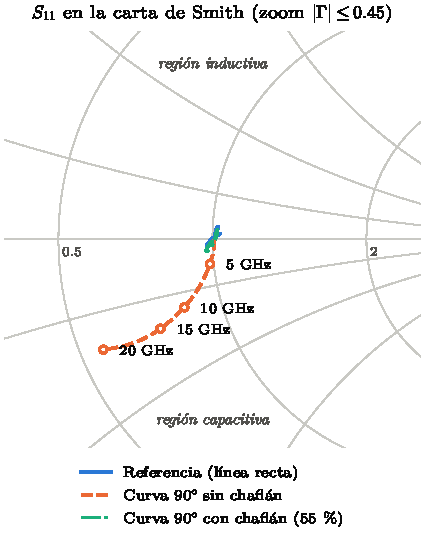
\includegraphics[width=0.5\textwidth]{figuras/fig4_Smith_S11.pdf}
\caption{Curva de \ang{90}: trayectoria de $S_{11}$ en la carta de Smith entre \SI{0.1}{} y \SI{20}{GHz}.}
\label{fig:smith}
\end{figure}

La Figura~\ref{fig:lc} y la Tabla~\ref{tab:lc} muestran los elementos extraídos con \eqref{eq:LC}. Entre 3 y \SI{12}{GHz} los valores son aproximadamente constantes, como corresponde a elementos concentrados. El resultado central es que la capacitancia de la esquina ($C=\SI{0.145}{pF}$) es prácticamente la misma que la de un tramo recto de igual área ($\SI{0.139}{pF}$), mientras que su inductancia por rama ($L=\SI{0.074}{nH}$) es menos de la mitad de la del tramo recto ($\SI{0.189}{nH}$). El chaflán hace lo contrario: reduce la capacitancia a \SI{0.077}{pF} y deja la inductancia casi igual (\SI{0.094}{nH}).

\begin{figure}[htbp]
\centering
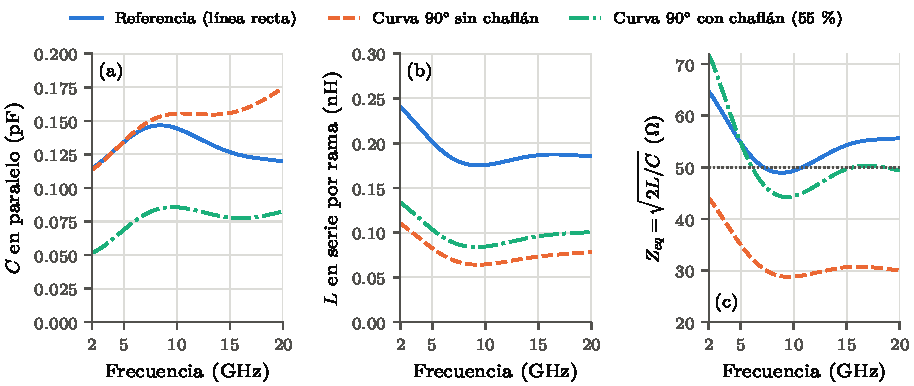
\includegraphics[width=\textwidth]{figuras/fig5_parasitos_LC.pdf}
\caption{Curva de \ang{90}: elementos del circuito equivalente en T extraídos de HFSS: (a) capacitancia en paralelo, (b) inductancia serie por rama y (c) impedancia local equivalente.}
\label{fig:lc}
\end{figure}

\begin{table}[htbp]
\centering
\caption{Curva de \ang{90}: circuito equivalente en T (promedio de 3 a \SI{12}{GHz}).}
\label{tab:lc}
\small
\begin{tabular}{lccccc}
\toprule
Diseño & $C$ (pF) & $L$ por rama (nH) & $Z_{eq}$ ($\Omega$) & $\tau$ (ps) & $|S_{11}|=-20$~dB en \\
\midrule
Referencia & 0.139 & 0.189 & 52.1 & -0.58 & $>\SI{20}{GHz}$ \\
Curva sin chaflán & 0.145 & 0.074 & 31.9 & 4.31 & \SI{7.00}{GHz} \\
Curva con chaflán & 0.077 & 0.094 & 49.8 & 0.10 & $>\SI{20}{GHz}$ \\
\bottomrule
\end{tabular}
\end{table}

\subsubsection{Transmisión y pérdida de inserción}
La Figura~\ref{fig:s21} muestra $|S_{21}|$. La curva sin compensar pierde \SI{0.26}{dB} a \SI{10}{GHz} y \SI{0.87}{dB} a \SI{20}{GHz}; la curva con chaflán, \SI{0.26}{dB} a \SI{20}{GHz}. Para saber de dónde viene esa pérdida se aplicó la separación \eqref{eq:separacion}; el resultado está en la Figura~\ref{fig:rad} y en la Tabla~\ref{tab:potencia}.

\begin{figure}[htbp]
\centering
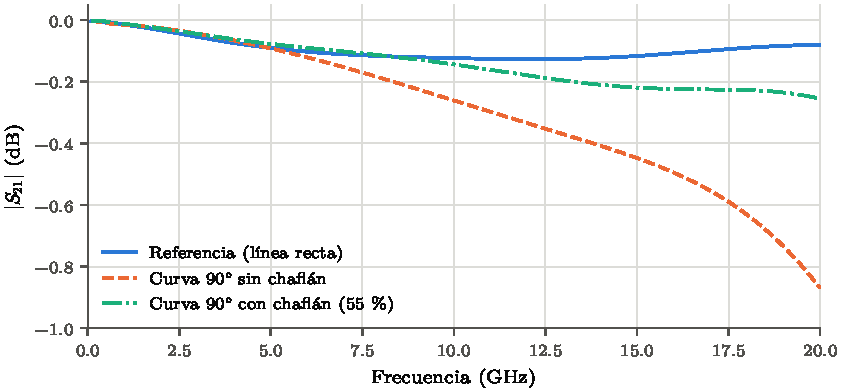
\includegraphics[width=\textwidth]{figuras/fig2_S21_dB.pdf}
\caption{Curva de \ang{90}: magnitud de $S_{21}$ (planos de referencia en los bordes de la esquina).}
\label{fig:s21}
\end{figure}

\begin{figure}[htbp]
\centering
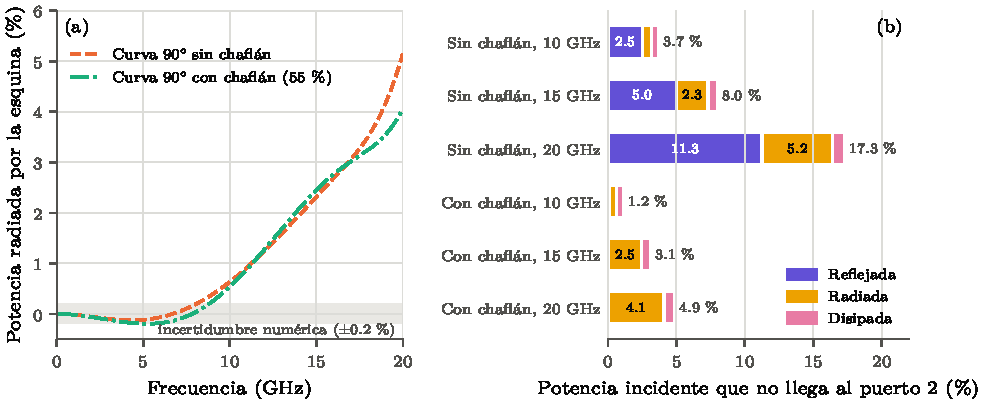
\includegraphics[width=\textwidth]{figuras/fig6_radiacion_potencia.pdf}
\caption{Curva de \ang{90}: (a) potencia radiada por la esquina, obtenida con \eqref{eq:separacion}; la banda gris es la incertidumbre numérica. (b) Destino de la potencia que no llega al puerto 2.}
\label{fig:rad}
\end{figure}

\begin{table}[htbp]
\centering
\caption{Curva de \ang{90}: destino de la potencia incidente (\%). El residuo es el error numérico común a todas las estructuras (pérdida aparente de la referencia sin pérdidas); incertidumbre de la radiada $\pm$0.2\,\%.}
\label{tab:potencia}
\small
\setlength{\tabcolsep}{4pt}
\begin{tabular}{lcccccccc}
\toprule
Diseño & $f$ (GHz) & Transmitida & Reflejada & Radiada & Disipada & Residuo & IL (dB) & IL$_{\mathrm{refl}}$ (dB) \\
\midrule
Sin chaflán & 10 & 94.2 & 2.5 & 0.6 & 0.6 & 2.1 & 0.26 & 0.11 \\
Sin chaflán & 15 & 90.2 & 5.0 & 2.3 & 0.7 & 1.8 & 0.45 & 0.22 \\
Sin chaflán & 20 & 81.9 & 11.3 & 5.2 & 0.9 & 0.8 & 0.87 & 0.52 \\
Con chaflán & 10 & 96.7 & 0.1 & 0.5 & 0.5 & 2.1 & 0.14 & 0.00 \\
Con chaflán & 15 & 95.1 & 0.0 & 2.5 & 0.7 & 1.8 & 0.22 & 0.00 \\
Con chaflán & 20 & 94.3 & 0.0 & 4.1 & 0.8 & 0.8 & 0.26 & 0.00 \\
\bottomrule
\end{tabular}
\end{table}

En la curva sin compensar la pérdida de inserción está dominada por la reflexión: a \SI{20}{GHz}, de los \SI{0.87}{dB}, \SI{0.52}{dB} se deben solo a la potencia reflejada. La radiación es despreciable por debajo de unos \SI{8}{GHz} y crece rápidamente, aproximadamente como $f^{3}$ entre 10 y \SI{20}{GHz}. La potencia disipada en cobre y dieléctrico es la misma en las tres estructuras dentro de la incertidumbre, de modo que la esquina no agrega pérdidas óhmicas apreciables.

\subsection{Discusión: explicación física}

\subsubsection{Por qué la esquina refleja}
\label{sec:d1porque}
Para ver qué ocurre dentro de la esquina se exportaron de HFSS los campos $\mathbf{E}$ y $\mathbf{H}$ a \SI{5}{GHz} en dos planos situados a \SI{0.02}{mm} por debajo y por encima de la traza. Con ellos se calcularon la densidad de carga superficial y la densidad de corriente superficial sobre la tira a partir de las condiciones de frontera en un conductor,
\begin{equation}
\rho_s = \varepsilon_0 E_z^{\mathrm{arriba}} - \varepsilon_0\varepsilon_r E_z^{\mathrm{abajo}}, \qquad
\mathbf{J}_s = \hat{\mathbf{z}}\times\left(\mathbf{H}^{\mathrm{arriba}}-\mathbf{H}^{\mathrm{abajo}}\right),
\label{eq:saltos}
\end{equation}
y se representaron en la Figura~\ref{fig:carga}. Se eligió \SI{5}{GHz}, por debajo del umbral de \SI{7}{GHz}, para observar la distribución que da origen a la reflexión.

\begin{figure}[htbp]
\centering
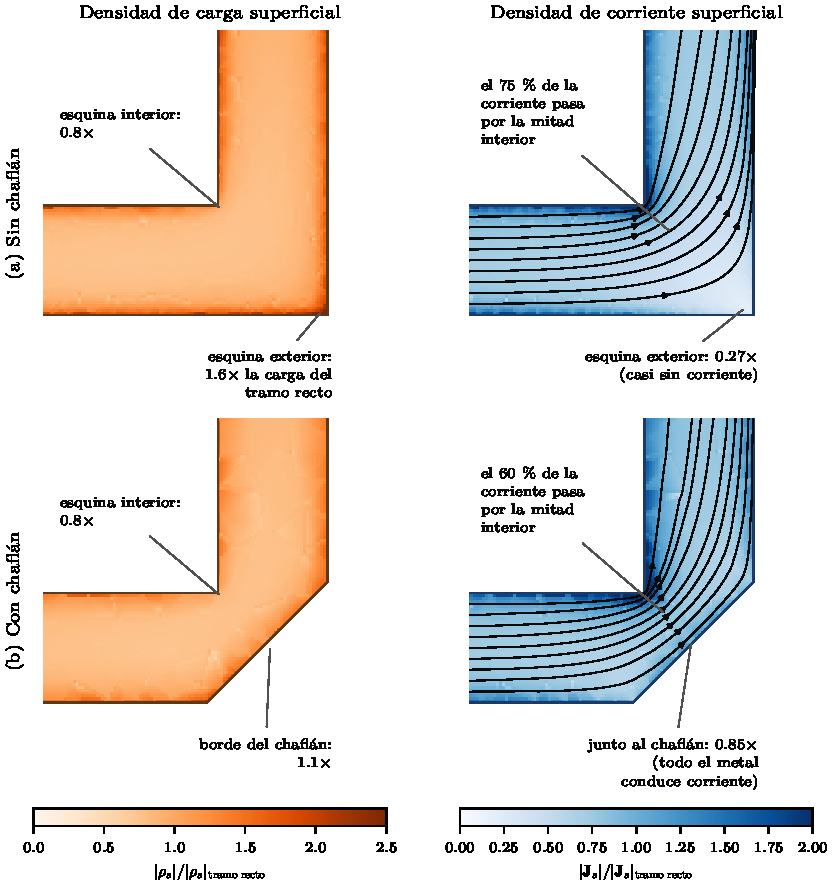
\includegraphics[width=\textwidth]{figuras/fig7_carga_corriente.pdf}
\caption{Curva de \ang{90}: densidad de carga superficial $|\rho_s|$ (izquierda) y densidad de corriente superficial $|\mathbf{J}_s|$ con sus líneas de flujo (derecha), calculadas con \eqref{eq:saltos} a partir de los campos de HFSS a \SI{5}{GHz}, para (a) la curva sin chaflán y (b) la curva con chaflán. Ambas están normalizadas a su promedio en una sección del brazo situada a $2.5W$ de la esquina; los factores indicados son promedios en un cuadrado de lado $W/4$ en cada esquina, o en una franja de ancho $W/4$ a lo largo del chaflán.}
\label{fig:carga}
\end{figure}

A lo ancho de la tira, tanto la carga como la corriente se concentran en los bordes, como corresponde a una línea a alta frecuencia. En la esquina, sin embargo, ambas se separan. En la curva sin chaflán (Figura~\ref{fig:carga}a) la esquina exterior tiene 1.6 veces la carga del tramo recto, pero solo 0.27 veces su corriente. Visto de otra forma, la mitad exterior del cuadrado de la esquina guarda el 60\,\% de su carga, mientras que el 75\,\% de la corriente que atraviesa la esquina pasa por la mitad interior de su diagonal; en un tramo recto ambos repartos serían de 50\,\%. La corriente toma el camino corto por la esquina interior, y la esquina exterior almacena carga, y por lo tanto energía eléctrica, casi sin corriente que la acompañe, y por lo tanto casi sin energía magnética.

En la curva con chaflán (Figura~\ref{fig:carga}b) ese metal ya no existe. La carga a lo largo del borde del chaflán es 1.1 veces la del tramo recto y la corriente junto a él 0.85 veces: todo el metal que queda conduce corriente, y la corriente se reparte de forma más pareja, con el 60\,\% por la mitad interior.

\paragraph{Consistencia con la extracción del circuito.} Sumando la carga dentro del cuadrado de la esquina se obtiene 0.99 veces la de un tramo recto de igual área, en acuerdo con el cociente de capacitancias extraído de los parámetros $S$ (1.04, Tabla~\ref{tab:lc}). Para la curva con chaflán ambos valores muestran la misma reducción fuerte (0.39 y 0.55). La coincidencia es menor porque la capacitancia de la red en T es un parámetro equivalente que reproduce los parámetros $S$ en los planos de referencia, y no exactamente la carga contenida en el cuadrado; la diferencia crece cuando la forma del metal se aleja de la de un tramo de línea, como con el chaflán, que deja solo el \SI{40}{\percent} del área del cuadrado.

En términos de \eqref{eq:poynting}, la región de la esquina almacena aproximadamente la misma energía eléctrica que un tramo recto de igual área, pero mucha menos energía magnética, porque la corriente recorre un camino más corto. El resultado es un exceso neto de energía eléctrica, es decir, un comportamiento capacitivo, que es exactamente lo que muestran la carta de Smith y la extracción de HFSS: $C$ igual a la del tramo recto y $L$ menor a la mitad.

Visto como línea de transmisión, el desequilibrio entre $L$ y $C$ equivale a insertar en la línea de \SI{50}{\ohm} un tramo corto de $Z_{eq}\approx\SI{32}{\ohm}$. Esa es la desadaptación de impedancias que produce la reflexión. El chaflán elimina justamente el metal de la esquina exterior, el que almacenaba carga sin conducir corriente; por eso reduce $C$ casi a la mitad sin cambiar mucho $L$, y restituye $Z_{eq}\approx\SI{50}{\ohm}$.

\subsubsection{A partir de qué frecuencia el efecto es significativo}
Se tomó como criterio de efecto significativo $|S_{11}|>-20$~dB, es decir, $|\Gamma|>0.1$, VSWR $>1.22$ o más del 1\,\% de la potencia reflejada. Con este criterio se distinguen tres regiones para la curva sin compensar:
\begin{itemize}
\item \textbf{Por debajo de unos \SI{4}{GHz}} la curva es indistinguible de la línea recta: su $|S_{11}|$ queda por debajo de \SI{-30}{dB}, al nivel de la referencia.
\item \textbf{Entre unos 4 y \SI{7}{GHz}} el efecto es medible pero pequeño.
\item \textbf{A partir de \SI{7.00}{GHz}} el efecto es significativo, y por encima de unos \SI{12}{GHz} se suma una radiación mayor al 1\,\%.
\end{itemize}

La explicación electromagnética está en \eqref{eq:poynting}. Mientras la esquina sea pequeña frente a $\lambda_g$, la distribución de campo en su vecindad es cuasiestática, y la diferencia de energías $W_m-W_e$ por unidad de $|I|^2$ es prácticamente independiente de la frecuencia. La reactancia neta, en cambio, lleva el factor $\omega$, y por eso crece linealmente con la frecuencia hasta que deja de ser despreciable frente a $Z_0$. Con el valor extraído $\tau=\SI{4.31}{ps}$, la ecuación \eqref{eq:gamma_tau} predice $|\Gamma|=0.1$ a
\[
f = \frac{0.1}{\pi\tau} = \SI{7.4}{GHz},
\]
en buen acuerdo con los \SI{7.00}{GHz} que da la simulación de onda completa.

\begin{figure}[htbp]
\centering
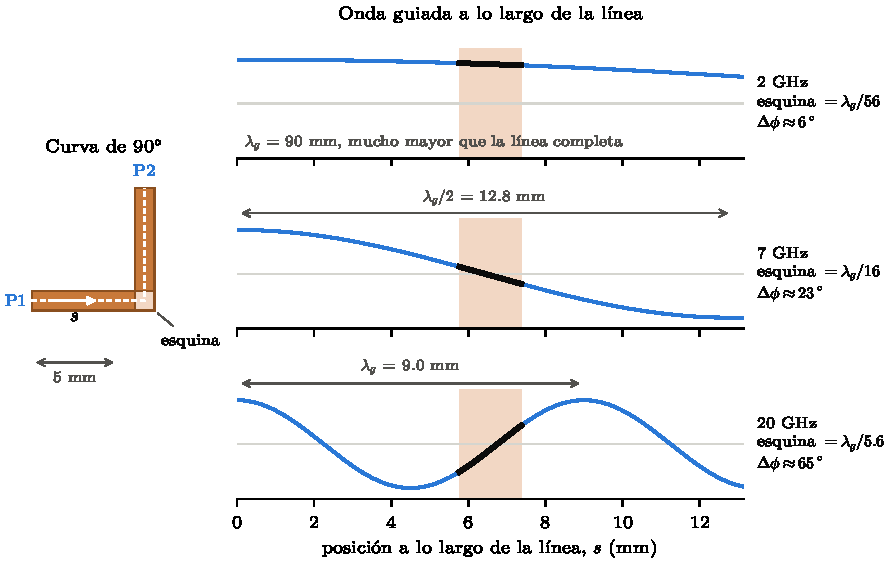
\includegraphics[width=\textwidth]{figuras/fig8_escala_lambda.pdf}
\caption{Tamaño de la esquina frente a la longitud de onda guiada. A la izquierda, la curva y la coordenada $s$ a lo largo del eje de la línea. A la derecha, una instantánea de la onda guiada, $\cos(2\pi s/\lambda_g)$, a 2, 7 y \SI{20}{GHz} en función de $s$. La franja marca la zona de la esquina (su diagonal, $W\sqrt{2}=\SI{1.61}{mm}$), el tramo negro es la parte de la onda que cae dentro de ella y $\Delta\phi$ es el desfase de la onda a través de la esquina.}
\label{fig:escala}
\end{figure}

La Figura~\ref{fig:escala} compara la esquina con la longitud de onda guiada $\lambda_g$. A \SI{2}{GHz} ($\lambda_g=\SI{90}{mm}$) la onda apenas cambia a lo largo de toda la estructura y la esquina mide $\lambda_g/56$: todos los puntos de la esquina ven prácticamente el mismo voltaje y la misma corriente al mismo tiempo. A \SI{7.00}{GHz}, donde el efecto se vuelve significativo, la esquina mide todavía $\lambda_g/16$ y la fase cambia solo \ang{23} a través de ella: la esquina sigue siendo eléctricamente pequeña y el modelo concentrado es válido. Esto muestra que el efecto no aparece porque la esquina sea ``grande'', sino porque el desequilibrio de energías multiplicado por $\omega$ deja de ser despreciable. A \SI{20}{GHz} ($\lambda_g=\SI{8.99}{mm}$) la esquina mide $\lambda_g/5.6$ y la fase cambia \ang{65} a través de ella. Ahí ya no puede tratarse como un punto: el modelo concentrado empieza a perder validez (la $C$ extraída deja de ser constante en la Figura~\ref{fig:lc}a) y la radiación crece rápidamente.

\subsubsection{Por qué el chaflán elimina la reflexión pero no la radiación}
\label{sec:d1rad}
Por el método de imágenes, la corriente $I$ de la tira y la corriente de retorno en el plano de tierra equivalen a dos corrientes opuestas, $I$ y $-I$, separadas $2h$ (Figura~\ref{fig:imagen}a). Lejos de la línea sus campos casi se anulan: el campo del par decae como $2h/r^2$ en lugar de $1/r$ (Figura~\ref{fig:imagen}b). Además, a lo largo de un tramo recto la onda viaja con $\beta=k_0\sqrt{\varepsilon_{\mathrm{eff}}}>k_0$, de modo que las contribuciones de los distintos elementos de corriente interfieren destructivamente en el espacio libre. Por ambas razones la línea recta guía la energía sin radiar.

\begin{figure}[htbp]
\centering
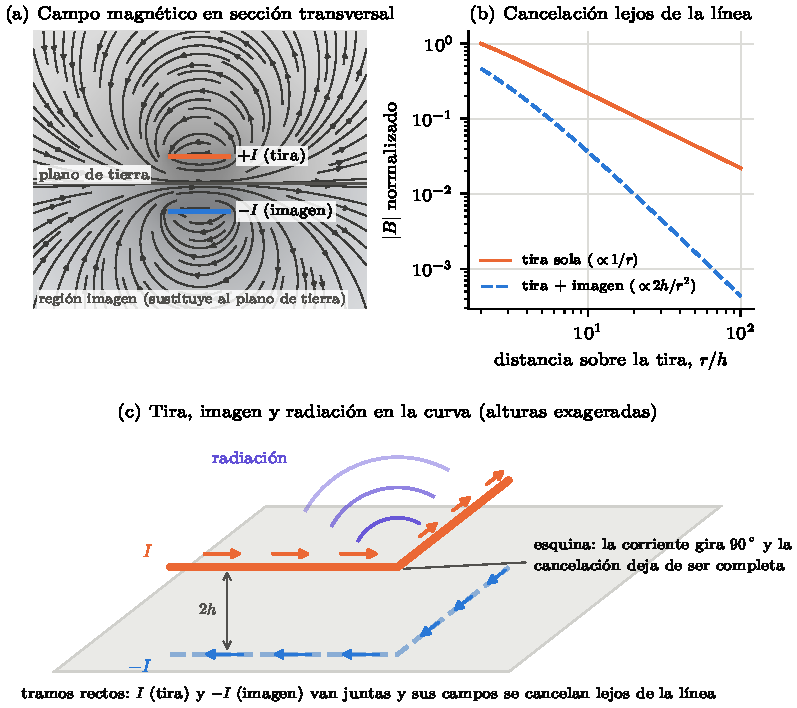
\includegraphics[width=\textwidth]{figuras/fig9_imagen_radiacion.pdf}
\caption{(a) Líneas de campo magnético de la tira y su imagen en sección transversal (el semiplano inferior es la región imagen que sustituye al plano de tierra). (b) Decaimiento del campo con la distancia para la tira sola y para el par tira--imagen. (c) Esquema de la curva: a lo largo de los tramos rectos $I$ y $-I$ viajan juntas; en la esquina la corriente gira \ang{90} y la cancelación deja de ser completa.}
\label{fig:imagen}
\end{figure}

En la esquina la corriente cambia de dirección bruscamente (Figura~\ref{fig:imagen}c). Las contribuciones de los dos brazos ya no apuntan en la misma dirección y no se compensan entre sí, de modo que la esquina radia como una pequeña antena \cite{lewin}. El chaflán corrige el exceso de carga, que es la causa de la reflexión, pero la corriente sigue girando \ang{90}; por eso ambas curvas radian cantidades similares (\SI{5.2}{\percent} y \SI{4.1}{\percent} a \SI{20}{GHz}). La radiación crece con la frecuencia y con el espesor eléctrico del sustrato, porque la separación $2h$ entre la tira y su imagen deja de ser despreciable frente a $\lambda_0$. En sustratos más gruesos o a frecuencias mayores sería el efecto dominante.

%======================================================================

%======================================================================
\section{Comparación entre discontinuidades}
\label{sec:comparacion}
La Tabla~\ref{tab:comparacion} resume las respuestas a la pregunta de investigación. Las cinco discontinuidades producen la reflexión por mecanismos distintos, y por eso dependen de la frecuencia de forma distinta. En la curva la línea es la misma de ambos lados y la reflexión la producen solo los parásitos, que crecen con $\omega$. En el cambio de ancho la reflexión la fija el cociente de impedancias y no depende de $\omega$. En el gap la conducción se interrumpe: la reflexión es casi total desde DC, y lo que crece con $\omega$ es la transmisión, a través del acoplamiento capacitivo. El cambio de sustrato es el caso más simple de todos: como la tira no cambia de forma, solo cambia $C'$ y la unión es un escalón de impedancia casi sin parásitos; la frecuencia interviene solo a través de la longitud eléctrica del tramo del otro material. El cambio de metal casi no refleja, y su efecto es una pérdida distribuida que crece como $\sqrt{f}$. La unión en T combina los dos tipos de mecanismo: una división de impedancias que refleja un tercio desde DC, como el cambio de ancho, y parásitos que crecen con $\omega$, como la curva, y que en este caso desequilibran el reparto de potencia.

Visto en conjunto, hay dos familias. En el cambio de ancho, el cambio de sustrato y la T, la reflexión principal es una diferencia de impedancias y está presente desde DC; la frecuencia solo importa a través de los parásitos o de la longitud eléctrica de un tramo. En la curva y en el divisor ya acoplado, la reflexión es solo parásita y aparece a partir de cierta frecuencia (\SI{7.00}{GHz} y \SI{13.0}{GHz}). El gap y el stub abierto son casos extremos. En el gap, el acoplamiento capacitivo es todo lo que une a las dos líneas, y la reflexión es casi total desde DC. En el stub, la rama abierta pone un corto en la línea en las frecuencias en que mide un número impar de cuartos de onda.

\begin{table}
\centering
\caption{Comparación entre las discontinuidades estudiadas.}
\label{tab:comparacion}
\footnotesize
\renewcommand{\arraystretch}{1}
\setlength{\tabcolsep}{3.5pt}
\newcolumntype{P}[1]{>{\raggedright\arraybackslash}p{#1}}
\begin{tabular}{P{3cm}P{6cm}}
\toprule
 & Curva de \ang{90}  \\
\midrule
Origen de la reflexión & Desequilibrio de energías almacenadas en la esquina (parásitos)\\
Dependencia con $f$ & $|\Gamma|\propto\omega$, nula en DC \\
$|S_{11}|>-20$~dB & A partir de \SI{7.00}{GHz} \\
Elementos parásitos & Capacitivos, dominan la respuesta \\
$|\Gamma|$ a \SI{20}{GHz} & 0.336 (VSWR 2.01) \\
Radiación a \SI{20}{GHz} & \SI{5.2}{\percent}, por el giro de la corriente  \\
Corrección o variante & Chaflán: elimina la reflexión en toda la banda, no la radiación \\
\bottomrule
\end{tabular}
\end{table}

\clearpage

\section{Limitaciones}
\begin{itemize}
\item El piso numérico de los puertos limita la reflexión más pequeña que se puede resolver: alrededor de $-30$~dB sin corregir. En la curva con chaflán solo puede afirmarse que $|S_{11}|<\SI{-30}{dB}$. En el cambio de ancho la corrección con las referencias lo reduce, y la asimetría residual entre $|S_{11}|$ y $|S_{22}|$ (0.007) indica su exactitud.
\item La radiación se obtiene por diferencia entre simulaciones y tiene una incertidumbre de $\pm\SI{0.2}{\percent}$ en la curva y $\pm\SI{0.3}{\percent}$ en el cambio de ancho.
\item La impedancia de una línea que no es TEM pura depende de su definición; en el cambio de ancho esto se manifiesta como una diferencia de \SI{2.3}{\percent} en el cociente $Z_2/Z_1$, absorbida por el parámetro $k$ del ajuste. Los datos fijan $C$ y $L_s$, pero no el reparto de $L_s$ entre ambos lados. En el cambio de sustrato, el escalón ideal se calculó con la impedancia $Z_{pi}$ de los puertos, y parte de la diferencia de hasta 0.019 por encima de \SI{10}{GHz} puede deberse a la misma ambigüedad.
\item Los conductores se modelaron con espesor cero y sin rugosidad superficial, por lo que la potencia disipada es una estimación aproximada.
\item En el gap, la reflexión casi total amplifica el error de $|S_{11}|$ en el balance de potencia, por lo que la radiación tiene una incertidumbre de $\pm\SI{0.7}{\percent}$; además, cinco de sus diseños llegaron al máximo de pases con un solo pase bajo el criterio. El reparto de líneas de campo se calculó en un solo corte vertical y es una medida cualitativa.
\item En el cambio de material, la reflexión de la unión cobre--estaño queda por debajo de la resolución de la corrección (\SI{-42}{dB}); solo puede afirmarse que es menor, y la comparación con \eqref{eq:gsn} es indirecta, a través de las atenuaciones de HFSS. El tramo finito de la Figura~\ref{fig:d4tramo} se calculó combinando parámetros $S$, lo que supone que los campos evanescentes de una unión no alcanzan a la otra; es válido para tramos de varios $h$ de largo.
\item El estaño se modeló como un conductor macizo de conductividad finita. Un acabado real es una capa de pocos micrómetros sobre el cobre: cuando su espesor es menor que unas cuantas profundidades de penetración (\SI{17}{\micro\metre} a \SI{0.1}{GHz}, \SI{5.4}{\micro\metre} a \SI{1}{GHz} y \SI{1.2}{\micro\metre} a \SI{20}{GHz}), parte de la corriente circula por el cobre y la pérdida queda entre la del cobre y la calculada aquí. Tampoco se modeló la rugosidad ni el cambio de espesor de la pista estañada.
\item Los sustratos se tomaron con $\varepsilon_r$ y $\tan\delta$ constantes con la frecuencia, y con el mismo espesor; en una placa real con dos laminados también cambian el espesor y, en el FR-4, la permitividad con la frecuencia.
\item En la unión en T, el modelo de Hammerstad se evaluó con las impedancias y permitividades efectivas de los puertos de HFSS y no con las fórmulas cuasi-estáticas originales, y el divisor, con una rama de \SI{1.14}{mm} sobre una línea de \SI{0.29}{mm}, está probablemente fuera del rango para el que se ajustó el modelo. La capacitancia en exceso de la T de \SI{50}{\ohm} solo es constante entre 2 y \SI{5}{GHz}; por encima, el circuito de una sola capacitancia no basta. La predicción del stub usa el extremo abierto de otro proyecto (la discontinuidad 3), simulado con la misma configuración, y supone que los campos de la unión y del extremo no interactúan. Los campos se exportaron solo a \SI{5}{GHz} y con una sola excitación por estructura.
\item Se estudió un solo sustrato base, una sola relación de anchos en el cambio de ancho, cinco separaciones en el gap, tres materiales en el cambio de material y una sola geometría de cada variante de la T; los valores numéricos dependen de $h$, $\varepsilon_r$ y la geometría, aunque los mecanismos físicos son generales.
\end{itemize}

\clearpage

\section{Conclusiones}

\textbf{Curva de \ang{90}.} La curva se comporta como una discontinuidad capacitiva: la esquina conserva la capacitancia de un tramo recto, pero la corriente la atraviesa por un camino más corto y su inductancia es menos de la mitad, por lo que equivale a un tramo corto de $\approx\SI{32}{\ohm}$ dentro de la línea de \SI{50}{\ohm}. Como la reactancia neta crece con $\omega$, la reflexión aumenta con la frecuencia y se vuelve significativa ($|S_{11}|>-20$~dB) a partir de \SI{7.00}{GHz}, cuando la esquina mide apenas $\lambda_g/16$. A frecuencias mayores se suma la radiación, causada por el cambio de dirección de la corriente.


\begin{thebibliography}{9}
\bibitem{pozar} D.~M. Pozar, \emph{Microwave Engineering}, 4th~ed. Hoboken, NJ, USA: Wiley, 2012.
\bibitem{gupta} K.~C. Gupta, R.~Garg, I.~Bahl y P.~Bhartia, \emph{Microstrip Lines and Slotlines}, 2nd~ed. Boston, MA, USA: Artech House, 1996.
\bibitem{douville} R.~J.~P. Douville y D.~S. James, ``Experimental study of symmetric microstrip bends and their compensation,'' \emph{IEEE Trans. Microw. Theory Techn.}, vol.~26, no.~3, pp.~175--182, 1978.
\bibitem{lewin} L.~Lewin, ``Radiation from discontinuities in strip-line,'' \emph{Proc. IEE, Part C}, vol.~107, no.~12, pp.~163--170, 1960.
\bibitem{rogers} Rogers Corporation, \emph{RO4000\textsuperscript{\textregistered} Series High Frequency Circuit Materials}, hoja de datos.
\bibitem{rogers3000} Rogers Corporation, \emph{RO3000\textsuperscript{\textregistered} Series Circuit Materials}, hoja de datos.
\bibitem{hammerstad} E.~Hammerstad, ``Computer-aided design of microstrip couplers with accurate discontinuity models,'' en \emph{IEEE MTT-S Int. Microwave Symp. Digest}, 1981, pp.~54--56.
\bibitem{qucs} S.~Jahn et al., \emph{Qucs Technical Papers}, sección ``Microstrip tee junction''. [En línea]. Disponible: \url{https://qucs.sourceforge.net/tech/node81.html}
\end{thebibliography}

\appendix
\section{Herramientas y métodos de cálculo}
\label{ap:metodos}

\subsection{Herramientas}
\begin{itemize}
\item \textbf{Ansys Electronics Desktop Student 2025~R2 (HFSS).} Solución de onda completa por elementos finitos en modo \emph{Driven Modal}. Los modelos no se dibujaron a mano: se construyeron, resolvieron y exportaron con scripts de la interfaz de automatización de AEDT escritos en Python. Para la curva: \texttt{P2\_D1\_Curva90\_v2.py} (seis estructuras), \texttt{P2\_Diagnostico\_Referencia.py} (variantes de la Tabla~\ref{tab:diag}) y \texttt{P2\_D1\_Exportar\_Campos.py} (campos de la Figura~\ref{fig:carga}). Para el cambio de ancho: \texttt{P2\_D2\_Escalon.py}, que construye las ocho estructuras, las resuelve, exporta los CSV y los campos y comprime los resultados; \texttt{P2\_D2\_Complemento.py} es el mismo script en modo complemento, que se usó para resolver con el límite de pases la transición sin pérdidas y agregar las referencias con pérdidas. Para el gap: \texttt{P2\_D3\_Gap.py}, que construye los doce diseños, los resuelve (y vuelve a resolver con menos pases cualquiera que exceda el límite de malla), exporta los CSV y los campos, incluido el corte vertical, y comprime los resultados. Para el cambio de material: \texttt{P2\_D4\_Material.py}, que construye los 16 diseños con sus materiales (incluidos el FR-4, el RO3010 y la conductividad del estaño), los resuelve uno por uno, exporta los CSV y los campos y comprime los resultados; \texttt{P2\_D4\_Reanudar.py} es el mismo script en modo de reanudación, que abre el proyecto existente y resuelve solo los diseños que aún no tienen resultados. Para la unión en T: \texttt{P2\_D5\_T.py}, que construye los 10 diseños (con tres puertos en la T y el divisor), los resuelve, exporta los CSV y los campos con la excitación indicada y comprime los resultados, \texttt{P2\_D5\_Reanudar.py}, su versión de reanudación, y \texttt{P2\_D5\_Campos\_Stub.py}, que agrega al stub tres puntos de frecuencia con campos guardados, los resuelve con la malla ya refinada y exporta los campos de las Figuras~\ref{fig:d5stubmapas} y~\ref{fig:d5stubonda}. Cada script crea las variables de diseño, la geometría, los materiales, las fronteras, los puertos, el análisis, las gráficas y la exportación de resultados.
\item \textbf{Python 3} con NumPy (aritmética compleja y álgebra lineal), SciPy (mínimos cuadrados no lineales, raíces e interpolación) y Matplotlib (figuras, exportadas como PDF vectorial). Con él se hizo todo el posprocesamiento y los cálculos auxiliares.
\item \textbf{\LaTeX} (pdflatex, con CircuiTikZ para los circuitos de las Figuras~\ref{fig:circescalon}, \ref{fig:circgap} y~\ref{fig:circt}). Las tablas y los valores numéricos citados en el texto se generan con un script directamente a partir de los datos de HFSS, sin transcripción manual.
\end{itemize}

El flujo de datos fue: HFSS $\rightarrow$ CSV y archivos de campo (parámetros $S$, impedancias y constantes de propagación de los puertos, balance de potencia, convergencia y campos $\mathbf{E}$ y $\mathbf{H}$) $\rightarrow$ Python (lectura, corrección, cálculo, figuras y tablas) $\rightarrow$ este documento. El código fuente se entrega junto con el reporte.

\subsection{Origen y método de cada figura y tabla}
\begin{description}[style=nextline,leftmargin=0pt,itemsep=4pt,font=\normalfont\bfseries]
\item[Sección~\ref{sec:diseno} (diseño de las líneas)] Evaluación numérica de \eqref{eq:eeff}, \eqref{eq:z0}, \eqref{eq:lg}, \eqref{eq:miter}, \eqref{eq:sintesis} y \eqref{eq:sintesis100}.

\item[Figura~\ref{fig:geo} (geometría)] Polígonos dibujados con Matplotlib a partir de las mismas dimensiones de los modelos de HFSS; el perfil de la transición se calcula con la misma rutina que usa el script de HFSS.

\item[Figura~\ref{fig:hfss3d} (modelos 3D)] Capturas del modelador 3D de HFSS.

\item[Tabla~\ref{tab:conv} (convergencia)] Exportación de la convergencia del análisis adaptativo de HFSS: número de tetraedros y $\max|\Delta S|$ del último pase.

\item[Tabla~\ref{tab:diag} (diagnóstico)] Balance \eqref{eq:balance} evaluado a \SI{10}{GHz} con los CSV de las variantes de la línea de referencia.

\item[Figuras~\ref{fig:s11}, \ref{fig:gamma} y \ref{fig:s21}; Tabla~\ref{tab:sparam}] $|S_{11}|$ y $|S_{21}|$ en dB del barrido interpolante de HFSS (399 puntos entre \SI{0.1}{} y \SI{20}{GHz}); $|\Gamma|=10^{S_{11}[\mathrm{dB}]/20}$ y VSWR por \eqref{eq:merito}.

\item[Figura~\ref{fig:smith} (carta de Smith)] $S_{11}$ complejo exportado de HFSS. La retícula se trazó con la transformación bilineal $\Gamma=(z-1)/(z+1)$ aplicada a las curvas de resistencia y reactancia normalizadas constantes.

\item[Figura~\ref{fig:lc} y Tabla~\ref{tab:lc} (circuito de la curva)] Para cada punto de frecuencia se reconstruyó $S_{21}$ complejo a partir de su magnitud y fase, se convirtió la matriz $S$ a parámetros $Z$ con \eqref{eq:zparam} y se calcularon $C$, $L$ y $Z_{eq}$ con \eqref{eq:LC}. La tabla promedia de 3 a \SI{12}{GHz}; $\tau$ se obtiene de \eqref{eq:gamma_tau}.

\item[Figura~\ref{fig:rad} y Tabla~\ref{tab:potencia} (potencia en la curva)] Balance \eqref{eq:balance} para cada estructura y su gemelo sin pérdidas, y separación \eqref{eq:separacion}. La incertidumbre es el máximo de $|P_{\mathrm{rad}}|$ por debajo de \SI{6}{GHz}, donde la radiación debe ser nula.

\item[Figura~\ref{fig:carga} (carga y corriente)] Campos $\mathbf{E}$ y $\mathbf{H}$ exportados de HFSS en un punto de frecuencia de \SI{5}{GHz} con campos guardados, en una malla regular (paso de \SI{0.03}{mm} en la curva y la transición, \SI{0.02}{mm} en el escalón y el gap) sobre los planos $z=h\pm\SI{0.02}{mm}$. Cada campo se exportó en fase \ang{0} y \ang{90} para reconstruir el fasor, $\mathbf{F}=\mathbf{F}(\ang{0})-j\,\mathbf{F}(\ang{90})$. Con \eqref{eq:saltos} se obtuvieron $\rho_s$ y $\mathbf{J}_s$ en los puntos que caen sobre la traza. En la curva, las líneas de flujo se trazan con la parte real de $\mathbf{J}_s$ en la fase de máxima corriente del brazo; en el cambio de ancho, con la parte de $\mathbf{J}_s$ en fase con la corriente total de cada sección, lo que quita el retardo de la onda a lo largo de la línea. Los repartos de la curva son la suma de $|\rho_s|$ en cada mitad del cuadrado de la esquina, separadas por la diagonal $x=y$, y la integral de $\mathbf{J}_s\cdot\hat{\mathbf{n}}$ a lo largo de la diagonal que une la esquina interior con la exterior, con interpolación bilineal. En el cambio de ancho, $q(x)$ es la suma de $\rho_s$ a lo ancho de la traza en cada sección; el escalón ideal es la recta ajustada a $q(x)$ en cada línea, lejos del escalón, extrapolada hasta el plano de unión; y la fracción de corriente es la suma de $|J_x|$ en $|y|<W_2/2$ entre la suma en todo el ancho.

\item[Figura~\ref{fig:escala} (escala de la onda)] $\lambda_g$ de \eqref{eq:lg} con $\varepsilon_{\mathrm{eff}}$ de \eqref{eq:eeff} (en la transición, el promedio de ambas líneas); onda $\cos(2\pi s/\lambda_g)$ y desfase $\Delta\phi=\ang{360}\,W\sqrt{2}/\lambda_g$. En la Figura~\ref{fig:descala}a el eje horizontal es $L_t/\lambda_g$ evaluado en cada frecuencia del barrido, y la teoría es \eqref{eq:taper}.

\item[Figura~\ref{fig:imagen} (tira e imagen)]
(a) Campo magnetostático bidimensional: la tira se representa con 41 corrientes filamentarias repartidas en su ancho y su imagen con las corrientes opuestas a una distancia $2h$; el campo es la superposición $\mathbf{B}\propto\sum_k I_k\,\hat{\mathbf{z}}\times(\mathbf{r}-\mathbf{r}_k)/|\mathbf{r}-\mathbf{r}_k|^2$. El color es $\log_{10}|\mathbf{B}|$ y las líneas son líneas de campo.
(b) $|\mathbf{B}|$ sobre el eje vertical de la tira para la tira sola y para el par tira--imagen.
(c) Esquema dibujado en proyección oblicua; es ilustrativo y no proviene de un cálculo.

\end{description}

\end{document}
